\cleardoublepage
\section{Souhrn}
    \begin{center}
        \makebox[\textwidth][c]{
            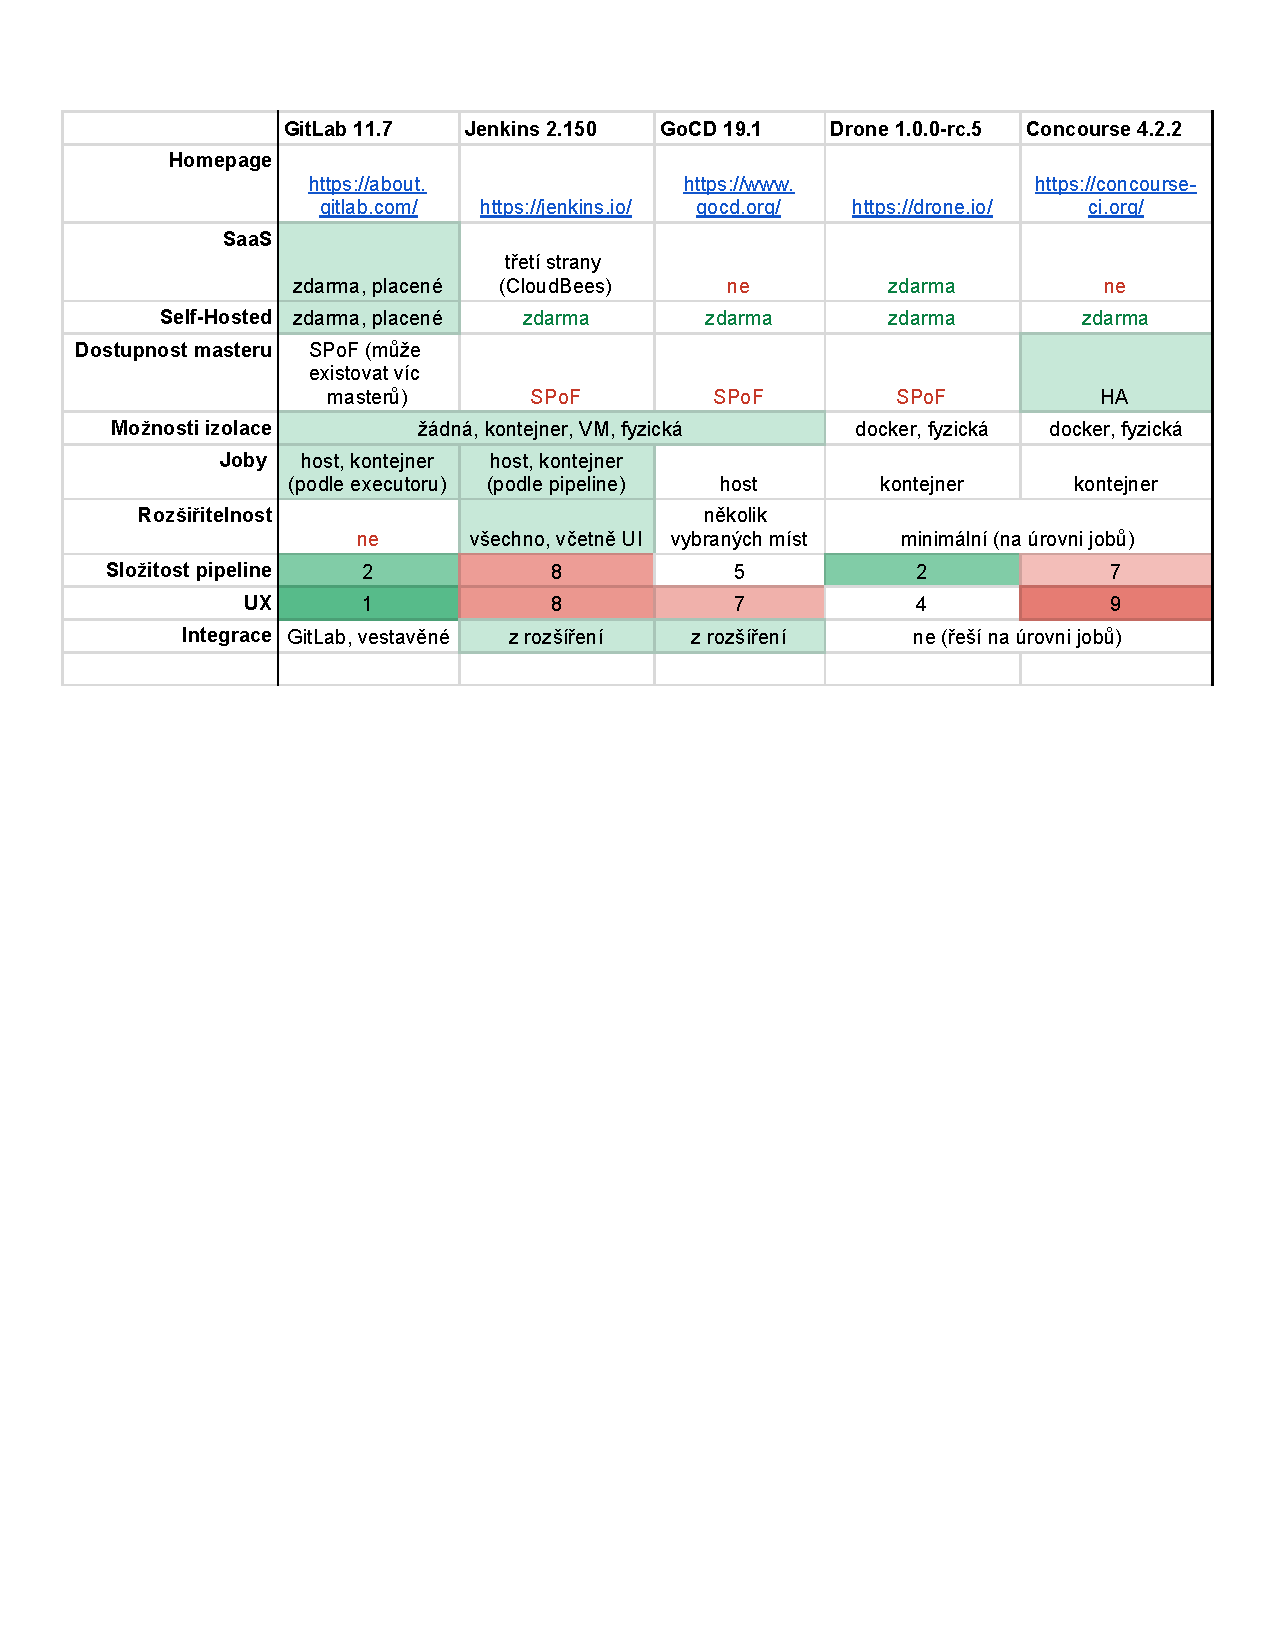
\includegraphics[page=1,width=1.4\textwidth]{media/porovnani-crop.pdf}
        }
    \end{center}

    \afterpage{
        \begin{center}
            \makebox[\textwidth][c]{
                \includegraphics[page=2,width=1.4\textwidth]{media/porovnani-crop.pdf}
            }
        \end{center}
    }

    Tabulka na této dvojstraně vizualizuje silné a slabé stránky porovnávaných \CI nástrojů. Zeleně podbarvené buňky reprezentují nejlepší hodnoty.

    S výjimkou GitLab jsou všechna \CI buď proprietární \glstext{SaaS} nebo zdarma, open-source a self-hosted. GitLab má odlišnou strategii a prodává licence i pro self-hosted variantu (GitLab \glstext{EE}).

    Dostupnost kontrolních serverů ma suverénně nejlepší Concourse, který umožňuje provozovat více masterů. GitLab může mít zaregistrováno více masterů (runnerů), ale každý se stará o svoji skupinu pipeline. Dostupnost agentů není uvedena. U všech \CI jsou joby stavové a z principu není možné je replikovat.

    Dále jsou \CI klasifikované podle úrovně izolace. Všechny self-hosted řešení nabízí izolaci kontejnery (ať už je přímo zabudovaná, je k dispozici pomocí rozšíření, nebo ji lze implementovat na úrovni samotného jobu). Díky master+agent architektuře lze také dosáhnout fyzické izolace, kde různí agenti běží na odlišných serverech. U \CI která nejsou postavená čistně na kontejnerech lze dosáhnout i žádné izolace. GitLab, Jenkins a GoCD ještě umožňují vytvářet dynamicky \glstext{VM}. U \glstext{SaaS} řešení která staví na kontejnerech není úplně jasné, jakou izolaci nabízí. Dá se ale očekávat, že uživatelé/organizace budou na oddělené \glstext{VM}.

    V řádku \textit{Joby} jsou porovnány možnosti konfigurace. U možnosti \textit{host} běží všechny příkazy na jedné \glstext{VM} a typicky nelze opakovat jenom části pipeline, ale konfigurace bývá intuitivnější. Oproti tomu varianta \textit{kontejner} označuje \CI, která rozdělují pipeline na různé části, kde každá se spouští v předem vytvořeném Docker kontejneru.

    Složitost pipeline a \glstext{UX} jsou čistě subjektivní relativní hodnocení. Škála je od 1 do 9, kde 1 je nejlepší skóre.

    \subsection{Použití jednotlivých \CI}
        \begin{description}
            \item[GitLab] Skvělé \CI. Podporuje jen repozitáře na GitLab. Dobrá podpora \CD.
            \item[Jenkins] Nejobecnější \CI s nejhorším \glstext{UX}. Použil bych až jako poslední možnost, pokud narazím na limitace jiných \CI.
            \item[GoCD] Funkčně stejné nebo horší než Jenkins, má menší komunitu, není tak udržovaný. Má nevýznamně lepší \glstext{UX}.
            \item[Drone] Minimalistické \CI. Využil bych pro cloud-ready organizace, které pracují výhradně s kontejnery.
            \item[Concourse] Alternativa ke Drone, má výrazně složitější konfiguraci a horší \glstext{UX}. Největši výhoda Concourse je vynikající dostupnost kontrolní roviny.
            \item[CircleCI] \glstext{SaaS} varianta Drone. Limitující faktor je cena. V rozhodování můžou hrát roli izolace a rychlost.
            \item[Travis CI] \glstext{SaaS} varianta \CI nezaloženého na kontejnerech.
            \item[Semaphore CI] Alternativa k Travis~CI s komplikovanější konfigurací, ale za lepší cenu.
            \item[GitHub Actions] Novinka, pravděpodobně bude používané jako doplněk k dalším \CI.
        \end{description}
